
    %!TeX program = lualatex
    \documentclass[12pt]{article}

    \usepackage[hmargin=0.5in, tmargin=0.75in, bmargin=0.9in]{geometry}
    \geometry{legalpaper, portrait}
   
    \usepackage{graphicx}  % graphic controls
    \usepackage{float}  % positioning controls
    \usepackage{lastpage}  % last page number finder
    \usepackage{makecell}  % helpers for multilined table cells

    % header/footer
    \usepackage{fancyhdr}
    \pagestyle{fancy}

    \lhead{2024 March 21}
    \chead{}
    \rhead{\footnotesize \thepage \ {\color{gray} of \pageref{LastPage}}}

    \cfoot{}
    \rfoot{\textbf{\LARGE Test Room}\\\vspace{3pt}{\large\color{gray}NIH STTR Phase II}}

    \renewcommand{\headrulewidth}{0.25pt}
    \renewcommand{\footrulewidth}{0.25pt}

    % drawing things
    \usepackage{tikz}
    \usetikzlibrary{math, calc, shapes, arrows.meta}

    \tikzstyle{grid-line} = [gray, very thin]
    \tikzstyle{wall} = [line width=2pt, line cap=round]
    \tikzstyle{window} = [line width=1pt, line cap=round]
    \tikzstyle{door} = [line width=1pt]
    \tikzstyle{furniture} = [draw, line width=0.5pt, transform shape]
    \tikzstyle{furniture-label} = [fill=white, align=center]
    \tikzstyle{sensor} = [circle, draw, color=teal, fill=teal, inner sep=0.5mm]
    \tikzstyle{sensor-label} = [fill=white, align=center, text=teal]
    \tikzstyle{location} = [diamond, draw, color=violet, fill=violet, inner sep=0.5mm]
    \tikzstyle{location-label} = [above, yshift=3pt, fill=white, text=violet]
    \tikzstyle{walking-path} = [densely dashed, line width=0.25mm, -{Stealth[length=4mm, width=2mm]}]
    \tikzstyle{nav-arrow} = [line width=0.25mm, {Stealth[length=4mm, width=2mm]}-, green!60!black]
    
    
    \def\furnitureR[height=#1, width=#2, rotate=#3](#4, #5){%
	% Draws a rectangular furniture piece centered on provided coordinates in a Tikz picture
	% \furnitureR[height=<value>, width=<value>, rotate=<degrees>](<x>, <y>)
	\draw[line width=2pt, color=black, rotate around={#3:(#4,#5)}] (#4-#2/2, #5-#1/2) rectangle (#4+#2/2, #5+#1/2)  
    }

    \def\furnitureC[radius=#1](#2, #3){%
	    % Draws a circular furniture piece centered on provided coordinates in a Tikz picture
	    % \furnitureC[radius=<value>](<x>, <y>)
	    \draw[line width=2pt, color=black] (#2, #3) circle (#1)
    }

    

    \def\camera[#1](#2,#3){
	    \node[circle, draw, color=blue!75!black, fill=blue!75!black, inner sep=0in, minimum size=0.1in, anchor=center, #1] at (#2,#3) {};
	    \node[isosceles triangle, draw, color=blue!75!black, fill=blue!75!black, inner sep=0in, minimum size=0.1in, isosceles triangle apex angle=75, anchor=east, #1] at (#2,#3) {}
     }

    \tikzstyle{camera-label} = [fill=white, align=center, text=blue!75!black]

    % units
    \usepackage{siunitx}
    \sisetup{per-mode = symbol}

    \let\DeclareUSUnit\DeclareSIUnit
    \let\US\SI
    \let\us\si
    \DeclareUSUnit\inch{in}
    \DeclareUSUnit\feet{ft}
    \DeclareUSUnit\foot{ft}
    \DeclareUSUnit\pound{lb}
    \DeclareUSUnit\slug{slug}

    % paragraph settings
    \setlength{\parindent}{0em}
    \raggedright

    \begin{document}
    \vspace*{.8in}
    \begin{figure}[H]
        \centering

        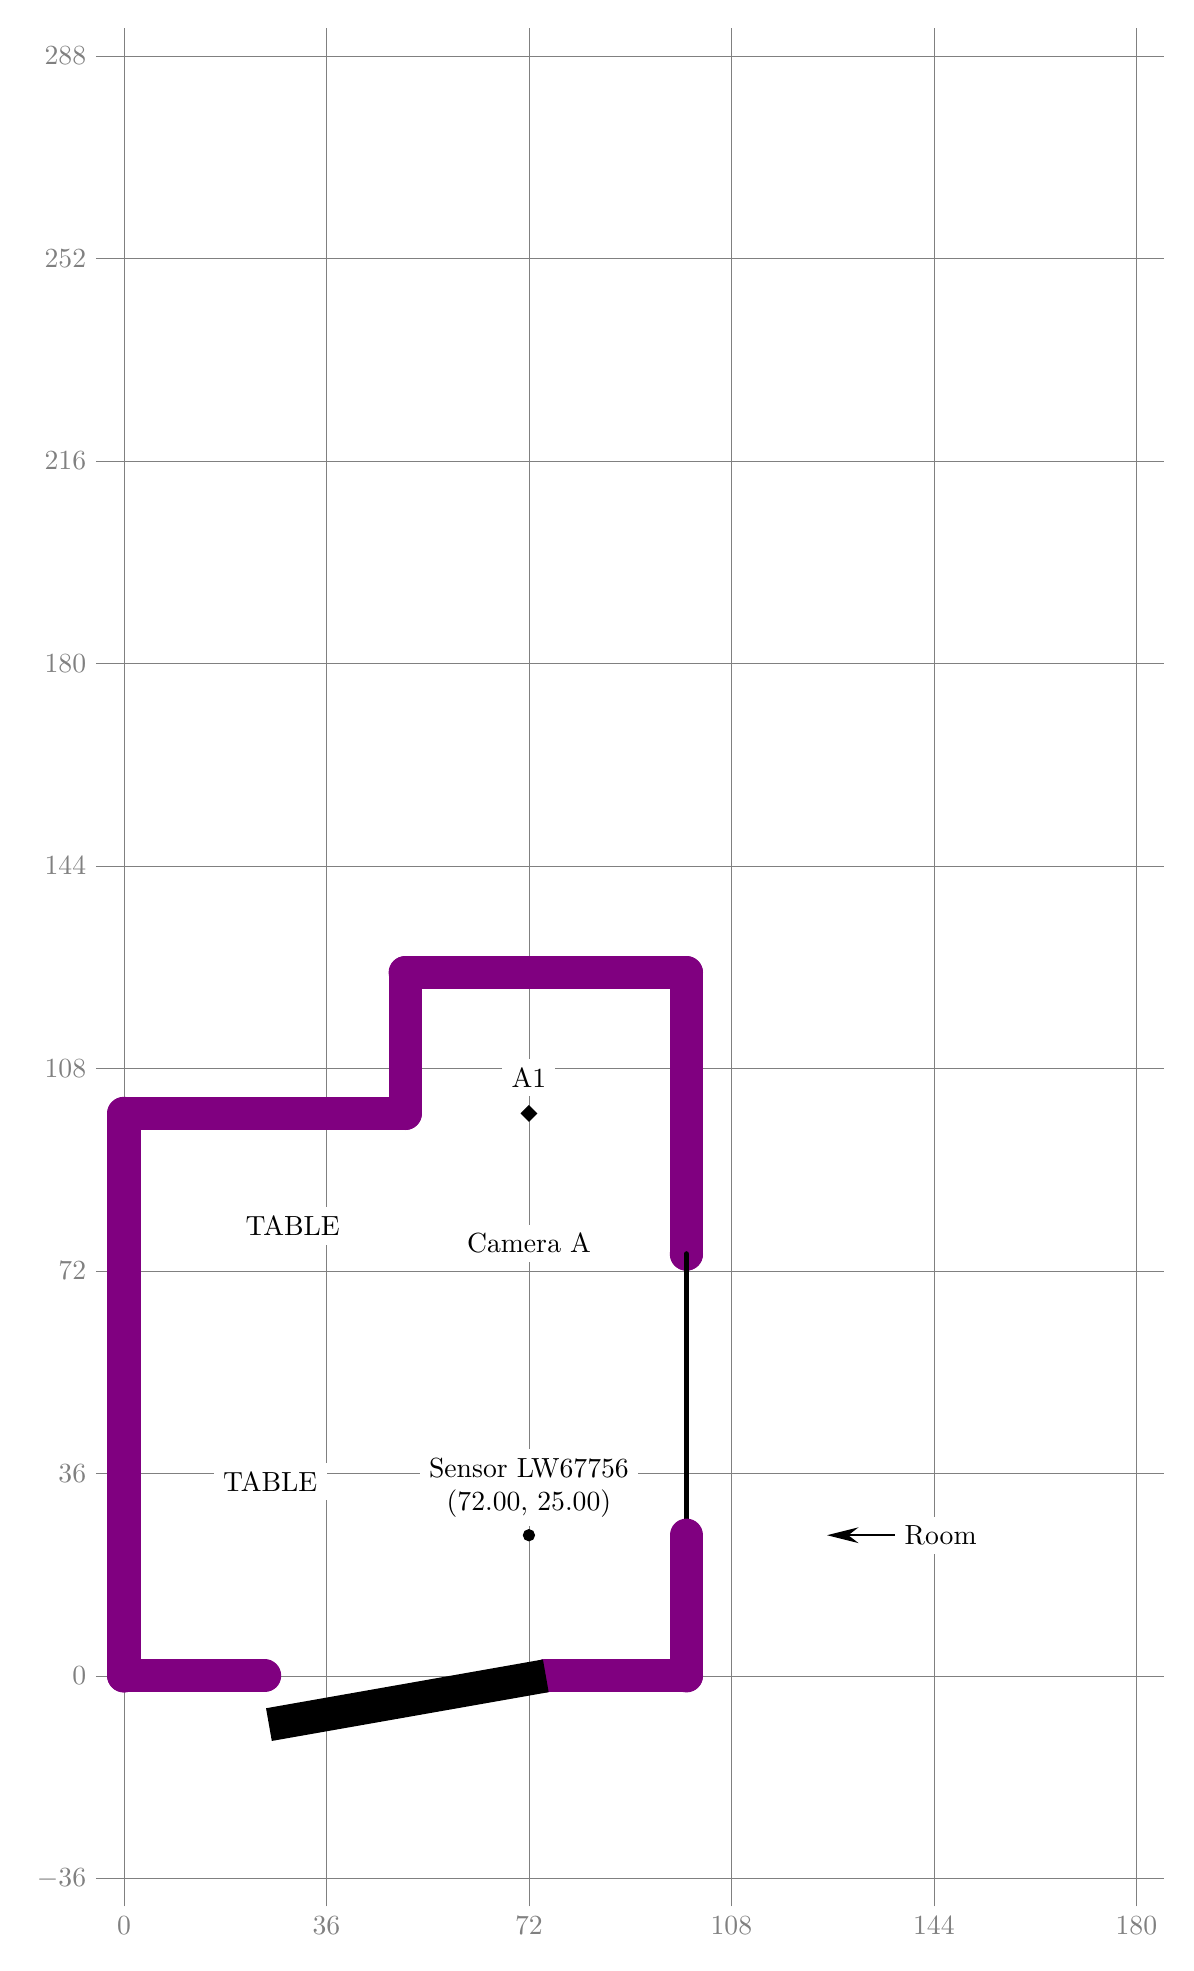
\begin{tikzpicture}[scale=1/14,  % use this to reduce or enlargen the image on paper
                            rotate=0]  % use this to rotate orientation by degrees on paper

    
        %% GRID - X
        \foreach \i in {0.0,36.0,...,180.0}{
            \draw[grid-line] (\i,-41.0) -- (\i,293.0);
            \tikzmath{int \value; \value = \i;}; 
            \node[gray, below] at (\i,-41.0) {\SI{\value}{\inch}};
        }

        %% GRID - Y
        \foreach \i in {-36.0,0.0,...,288.0}{
            \draw[grid-line] (-5.0,\i) -- (185.0,\i);
            \tikzmath{int \value; \value = \i;};
            \node[gray, left] at (-5.0,\i) {\SI{\value}{\inch}};
        }
    

    \node[location, color=black](A1) at (72.0,100.0) {};
\node[location-label,above,yshift=3pt, text=black] at (A1) {A1};
\camera[color=black,rotate=90.0](72.0,72.0);
\node[camera-label,yshift=3pt,above, text=black] at (72.0,72.0) {Camera A};
\node[sensor, color=black](sensor) at (72.0,25.0) {};
\node[sensor-label,yshift=3pt,above,text=black] at (72.00,25.00) {Sensor LW67756 \\ (72.00, 25.00)};
\furnitureR[height=24.0, width=24.0, rotate=0.0](26.0, 34.5);
\node[furniture-label, text=black ] at (26.0,34.5) {TABLE};
\furnitureC[radius=10.0](30.0, 80.0);
\node[furniture-label, text=black ] at (30.0,80.0) {TABLE};
\draw[wall, line width=12pt,color =violet] (0.00,0.00) -- (0.00,100.00) coordinate (c);
\draw[wall, line width=12pt,color =violet] (0.00,100.00) -- (50.00,100.00) coordinate (c);
\draw[wall, line width=12pt,color =violet] (50.00,100.00) -- (50.00,125.00) coordinate (c);
\draw[wall, line width=12pt,color =violet] (50.00,125.00) -- (100.00,125.00) coordinate (c);
\draw[wall, line width=12pt,color =violet] (100.00,125.00) -- (100.00,75.00) coordinate (c);
\draw[wall, line width=12pt,color =violet] (100.00,75.00) -- (100.00,75.00) coordinate (c);
\draw[window,line width=2pt, color=black] (100.00,75.00) -- (100.00,25.00) coordinate (c);
\draw[window,line width=2pt, color=black] (100.00,25.00) -- (100.00,25.00) coordinate (c);
\draw[wall, line width=12pt,color =violet] (100.00,25.00) -- (100.00,0.00) coordinate (c);
\draw[wall, line width=12pt,color =violet] (100.00,0.00) -- (75.00,0.00) coordinate (c);
\draw[wall, line width=12pt,color =violet] (75.00,0.00) -- (75.00,0.00) coordinate (c);
\draw[door, rotate around={10.00:(75.00,0.00)}, line width=12pt, color=black] (75.00,0.00) -- ++(-50.00,0.00);
\draw[wall, line width=12pt,color =violet] (25.00,0.00) -- (0.00,0.00) coordinate (c);
\draw[wall, line width=12pt,color =violet] (0.00,0.00) -- (0.00,0.00) coordinate (c);
\draw[nav-arrow,color=black] (125.0,25.0) -- ++(12,0) node[right, fill=white] {Room};


    
    \end{tikzpicture}
    \end{figure}
    
    \vspace*{\fill}  % fills the area between the table and layout with whitespace, forcing the table to the bottom of the page.
    \begin{table}[H]
	\begin{tabular}{l l}
		\makecell[lt]{
			\textbf{Location:}\\
     		Broad Neighborhood \\
 		    Greenway Bldg, Still Hopes\\
           	1 Still Hopes Drive\\
           	West Columbia, SC 29033\\\\
        }   	
        &	
		\makecell[tp{5in}]{
		\textbf{Notes:}\\
		\vspace{-8mm}  % reduce whitespace created by itemize above list
		\begin{itemize}
			\setlength\itemsep{-3mm}  % reduce whitespace created by itemize between lines
			\item Measurements are to the nearest \SI{0.25}{\inch}
			\item The furniture locations are approximate.
			\item Laptop and data acquisition system is located beside the table.
			\item Cameras are located on the ceiling.
		\end{itemize}
		}	
			
	\end{tabular}
	\vspace{-8mm} % reduce whitespace after table
\end{table}

    \end{document}
    